% ============================================================
% 3.2.3.2 Employment and Unemployment
% AQA AS Economics
% Sources: output/authoritative/as_syllabus.json (3.2.3.2)
%          output/authoritative/sow.json (as > 3.2 > 3.2.3)
% Suggested timing: 5 hours
% ============================================================

\documentclass[16pt,aspectratio=169]{beamer}
\usetheme{Madrid}
\usecolortheme{default}

\usepackage{graphicx}
\graphicspath{{../../../../../assets/images/}{./figures/}}
\usepackage{booktabs}
\usepackage{tikz}
\usepackage{pgfplots}
\pgfplotsset{compat=1.18}
\RequirePackage{tcolorbox}
\tcbuselibrary{skins}

% Key Point — yellow; for the single most important idea on a slide
\newtcolorbox{keypoint}{
    enhanced,
    colback=yellow!12,
    colframe=yellow!60!black,
    fonttitle=\bfseries,
    title=Key Point,
    arc=2pt,
    boxrule=0.8pt,
}

% Formula — blue; for named equations and their variable key
\newtcolorbox{formula}[1][Formula]{
    enhanced,
    colback=blue!5,
    colframe=blue!45!black,
    fonttitle=\bfseries,
    title=#1,
    arc=2pt,
    boxrule=0.8pt,
}

% Example Question — teal; for exam-style questions posed to students
\newtcolorbox{examplequestion}[1][Example Question]{
    enhanced,
    colback=teal!6,
    colframe=teal!55!black,
    fonttitle=\bfseries,
    title=#1,
    arc=2pt,
    boxrule=0.8pt,
}

% Example Solution — green; always follows an examplequestion block
\newtcolorbox{examplesolution}[1][Solution]{
    enhanced,
    colback=green!6,
    colframe=green!45!black,
    fonttitle=\bfseries,
    title=#1,
    arc=2pt,
    boxrule=0.8pt,
}

% ---- Worksheet environments --------------------------------

% Scenario — blue; for group discussion prompts on worksheets
% Usage: \begin{scenario}{Scenario 1: Title with commas, fine} ... \end{scenario}
\newtcolorbox{scenario}[1]{
    enhanced,
    colback=blue!5,
    colframe=blue!45!black,
    fonttitle=\bfseries,
    title={#1},
    arc=2pt,
    boxrule=0.8pt,
}

% Instructions — blue; for worksheet-level instruction blocks
\newtcolorbox{instructions}{
    enhanced,
    colback=blue!5,
    colframe=blue!45!black,
    fonttitle=\bfseries,
    title=Instructions,
    arc=2pt,
    boxrule=0.8pt,
}

% Extract — grey; for data response source material
% Usage: \begin{extract}{Source: Author, Year} ... \end{extract}
\newtcolorbox{extract}[1]{
    enhanced,
    colback=gray!8,
    colframe=gray!50,
    fonttitle=\bfseries,
    title={#1},
    arc=2pt,
    boxrule=0.8pt,
}


\title{Employment and Unemployment}
\subtitle{3.2.3.2 | AQA AS Economics}
\author{Dr Jac Thomas}
\date{\today}

\begin{document}

% ---- Title -------------------------------------------------
\begin{frame}
    \titlepage
\end{frame}

% ---- Learning Objectives -----------------------------------
\begin{frame}{Learning Objectives}
    \textbf{To be able to\ldots}
    \begin{itemize}
        \item Explain the two main UK measures of unemployment and distinguish between them
        \item Define and distinguish between the four types of unemployment
        \item Analyse how demand-side and supply-side factors determine employment and unemployment
        \item Explain how changes in the rest of the world affect UK employment
        \item Use AD/AS diagrams to illustrate unemployment
        \item Apply the ``symptoms, diagnosis, prescription'' technique to unemployment problems
    \end{itemize}
\end{frame}

% ---- What is Unemployment? ---------------------------------
\begin{frame}{What is Unemployment?}
    \begin{definition}
        \textbf{Unemployment} occurs when people of working age are without a job but are actively seeking work.
    \end{definition}

    \vspace{0.8em}
    \textbf{Why does it matter?}
    \begin{itemize}
        \item Lost output: the economy produces below its productive potential
        \item Cost to individuals: lost income, wellbeing, and skills
        \item Fiscal cost: government pays more in benefits, receives less in tax
        \item A key macroeconomic policy objective is to keep unemployment low
    \end{itemize}

    \vspace{0.5em}
    \begin{keypoint}
        Unemployment has a variety of causes. Appropriate policies to reduce it depend on correctly identifying the cause --- like a doctor diagnosing before prescribing.
    \end{keypoint}
\end{frame}

% ---- Measuring Unemployment --------------------------------
\begin{frame}{Measuring Unemployment: Two Official Measures}
    The UK uses two main measures of unemployment:

    \vspace{0.8em}
    \begin{columns}
        \begin{column}{0.47\textwidth}
            \textbf{1. Claimant Count}
            \begin{itemize}
                \item Counts those claiming unemployment-related benefits (mainly Universal Credit)
                \item Published monthly
                \item Easy to collect --- administrative data
                \item Affected by changes in benefit rules
            \end{itemize}
        \end{column}
        \begin{column}{0.47\textwidth}
            \textbf{2. Labour Force Survey (LFS)}
            \begin{itemize}
                \item Uses the ILO definition: without work, actively sought in last 4 weeks, available to start within 2 weeks
                \item Published quarterly
                \item Internationally comparable
                \item Based on a sample survey
            \end{itemize}
        \end{column}
    \end{columns}
\end{frame}

% ---- Claimant Count ----------------------------------------
\begin{frame}{The Claimant Count}
    \begin{definition}
        The \textbf{claimant count} measures the number of people claiming unemployment-related benefits, principally Universal Credit.
    \end{definition}

    \vspace{0.6em}
    \textbf{Limitations:}
    \begin{itemize}
        \item Excludes unemployed people not entitled to or not claiming benefits
        \item Changes in benefit rules alter the count even if unemployment hasn't changed --- it is not a pure labour market measure
        \item Tends to \textbf{undercount} true unemployment
    \end{itemize}

    \vspace{0.4em}
    \begin{example}
        When the UK moved from Jobseeker's Allowance to Universal Credit, the claimant count rose sharply --- not because unemployment increased, but because the eligibility criteria changed.
    \end{example}
\end{frame}

% ---- Labour Force Survey -----------------------------------
\begin{frame}{The Labour Force Survey (LFS)}
    \begin{definition}
        The \textbf{Labour Force Survey (LFS)} uses the ILO definition: a person is unemployed if they are (1) without a job, (2) have actively sought work in the last four weeks, and (3) are available to start work within two weeks.
    \end{definition}

    \vspace{0.4em}
    \textbf{Advantages over the claimant count:}
    \begin{itemize}
        \item Not distorted by benefit eligibility changes
        \item Internationally comparable (ILO standard used worldwide)
        \item Captures unemployed people not claiming benefits
    \end{itemize}

    \vspace{0.3em}
    \textbf{Limitation:} Based on a sample survey --- subject to sampling error.

    \vspace{0.3em}
    \textbf{The LFS is the UK's preferred headline measure.} The claimant count is still reported but harder to interpret due to changing benefit rules.
\end{frame}

% ---- Quantitative Skills -----------------------------------
\begin{frame}{Quantitative Skills: Reading Unemployment Data}
    You need to convert unemployment numbers into \textbf{rates}, calculate \textbf{absolute} and \textbf{percentage changes}, and interpret \textbf{index numbers}.

    \vspace{0.4em}
    \begin{examplequestion}
        In January 2024, LFS unemployment was 1.50 million and the UK labour force was 34.0 million.
        (a) Calculate the unemployment rate. (b) If unemployment rose by 85,000 the following month, calculate the new rate.
    \end{examplequestion}

    \vspace{0.3em}
    \begin{examplesolution}
        (a) $\dfrac{1{,}500{,}000}{34{,}000{,}000} \times 100 = \mathbf{4.4\%}$

        \vspace{0.3em}
        (b) $\dfrac{1{,}585{,}000}{34{,}000{,}000} \times 100 = \mathbf{4.7\%}$
    \end{examplesolution}
\end{frame}

% ---- Types of Unemployment: Overview -----------------------
\begin{frame}{Four Types of Unemployment}
    \begin{keypoint}
        Unemployment has a variety of causes. Identifying the type is essential before recommending a policy solution.
    \end{keypoint}

    \vspace{0.4em}
    \begin{table}
        \centering
        \renewcommand{\arraystretch}{1.15}
        \begin{tabular}{@{}p{2.8cm}p{6.0cm}p{4.0cm}@{}}
            \toprule
            \textbf{Type} & \textbf{Cause} & \textbf{Example} \\ \midrule
            Frictional  & Workers between jobs; search frictions & Graduate job hunting \\
            Structural  & Skill/geographic mismatch; industry decline & Tata Steel, Port Talbot \\
            Cyclical    & Deficient aggregate demand (recession) & 2008 financial crisis \\
            Seasonal    & Predictable variation in labour demand & Tourism, agriculture \\ \bottomrule
        \end{tabular}
    \end{table}
\end{frame}

% ---- Frictional --------------------------------------------
\begin{frame}{Frictional Unemployment}
    \begin{definition}
        \textbf{Frictional unemployment} arises from the time it takes workers to find a new job when moving between employment. It exists even when vacancies are available.
    \end{definition}

    \vspace{0.3em}
    \textbf{Causes:}
    \begin{itemize}
        \item Imperfect information: workers and employers are not instantly matched
        \item Workers take time to search for the right job at the right wage
        \item Geographical immobility may slow the search process
    \end{itemize}

    \vspace{0.2em}
    \textbf{Policy:} Improve job matching (better job centres, online platforms); reduce information asymmetries.

    \vspace{0.2em}
    \begin{example}
        A developer resigns to find a better-paid role. She accepts an offer after six weeks --- frictionally unemployed throughout, despite vacancies existing.
    \end{example}
\end{frame}

% ---- Structural --------------------------------------------
\begin{frame}{Structural Unemployment}
    \begin{definition}
        \textbf{Structural unemployment} results from a long-run mismatch between the skills workers have and the skills employers need, typically caused by the permanent decline of industries.
    \end{definition}

    \vspace{0.3em}
    \textbf{Causes:}
    \begin{itemize}
        \item Deindustrialisation: whole sectors shrink (steel, coal, shipbuilding)
        \item Technological change: automation displaces workers
        \item Occupational and geographical immobility slow re-employment
    \end{itemize}

    \vspace{0.2em}
    \textbf{Policy:} Retraining; education; regional investment; improving labour mobility.

    \vspace{0.2em}
    \begin{example}
        In 2024, Tata Steel cut 2,800 jobs at Port Talbot. Workers face structural unemployment: steelmaking skills have little local demand and geographical mobility is low.
    \end{example}
\end{frame}

% ---- Cyclical ----------------------------------------------
% Curve equations and intersections (pre-calculated):
%   SRAS: P = 0.8Y
%   AD:   P = 9 - Y   =>  Ye: Y=5, P=4
%   LRAS: Y = 7             Yf = 7
%   xmax = 9.5 (≥ Yf × 1.25)
\begin{frame}{Cyclical Unemployment}
    \begin{columns}
        \begin{column}{0.55\textwidth}
            \begin{center}
                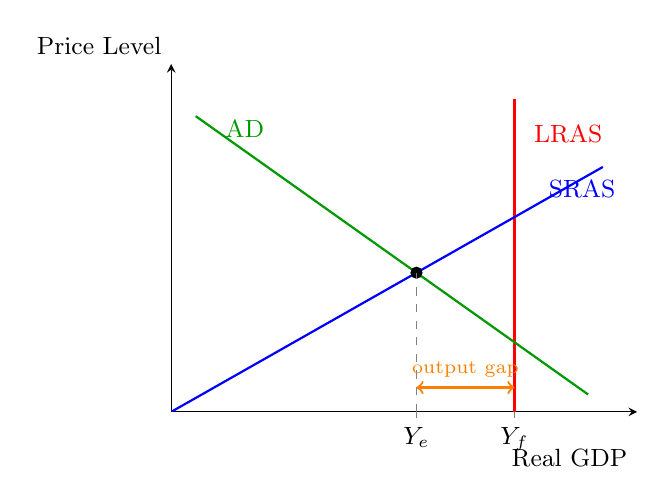
\begin{tikzpicture}
                    \begin{axis}[
                        axis lines = middle,
                        xmin=0, xmax=9.5, ymin=0, ymax=10,
                        xtick={5, 7},
                        xticklabels={$Y_e$, $Y_f$},
                        ytick=\empty,
                        width=7.5cm, height=6cm,
                        xlabel={Real GDP},
                        ylabel={Price Level},
                        xlabel style={at={(axis description cs:1,0)}, anchor=north east, yshift=-10pt, font=\small},
                        ylabel style={at={(axis description cs:0,1)}, anchor=south east, font=\small},
                        tick label style={font=\small},
                    ]
                    % LRAS at Yf=7; label to the right of line at mid-height (anchor=west)
                    \addplot[red, thick] coordinates {(7,0) (7,9.0)};
                    \node[red, font=\small, anchor=west] at (axis cs: 7.2, 8.0) {LRAS};
                    % SRAS: P=0.8Y; label above curve at x=7.5 (anchor=west, within xmax)
                    \addplot[blue, thick, domain=0:8.8] {0.8*x};
                    \node[blue, font=\small, anchor=west] at (axis cs: 7.5, 6.4) {SRAS};
                    % AD: P=9-Y; label above upper-left portion (anchor=south)
                    \addplot[green!60!black, thick, domain=0.5:8.5] {9 - x};
                    \node[green!60!black, font=\small, anchor=south] at (axis cs: 1.5, 7.6) {AD};
                    % Equilibrium E (Y=5, P=4); dashed drop to x-axis confirms tick alignment
                    \coordinate (E) at (axis cs: 5, 4);
                    \filldraw (E) circle (2pt);
                    \draw[dashed, gray] (axis cs: 5, 0) -- (E);
                    % Output gap: bracket from Ye to Yf
                    \draw[<->, thick, orange]
                        (axis cs: 5, 0.7) -- node[above, font=\scriptsize]{output gap} (axis cs: 7, 0.7);
                    \end{axis}
                \end{tikzpicture}
            \end{center}
        \end{column}
        \begin{column}{0.42\textwidth}
            \begin{definition}
                \textbf{Cyclical} (Keynesian) \textbf{unemployment} is caused by a fall in aggregate demand, leaving the economy below its productive potential.
            \end{definition}
            \vspace{0.5em}
            \begin{itemize}\setlength\itemsep{0.35em}
                \item Rises in recessions, falls in booms
                \item AD $\downarrow$ $\Rightarrow$ output $\downarrow$ $\Rightarrow$ firms hire fewer workers
                \item Negative output gap: $Y_e < Y_f$
                \item \textbf{Policy:} expansionary fiscal or monetary policy to boost AD
            \end{itemize}
        \end{column}
    \end{columns}
\end{frame}

% ---- Seasonal ----------------------------------------------
\begin{frame}{Seasonal Unemployment}
    \begin{definition}
        \textbf{Seasonal unemployment} occurs when demand for labour varies predictably with the time of year, leaving workers unemployed during the off-season.
    \end{definition}

    \vspace{0.8em}
    \textbf{Common sectors:}
    \begin{itemize}
        \item Tourism and hospitality: hotels and restaurants quiet in winter
        \item Agriculture: harvest work concentrated in summer/autumn
        \item Retail: temporary Christmas staff laid off in January
        \item Construction: activity falls in severe winter weather
    \end{itemize}

    \vspace{0.5em}
    \textbf{Note:} Seasonal unemployment is relatively minor compared to structural or cyclical unemployment. The ONS publishes \textbf{seasonally adjusted} figures to strip this out and show the underlying trend.
\end{frame}

% ---- Demand-Side Factors -----------------------------------
\begin{frame}{Demand-Side Causes of Unemployment}
    Firms hire workers to produce output. When aggregate demand falls, they need fewer workers --- causing \textbf{cyclical unemployment}.

    \vspace{0.4em}
    \textbf{Key demand-side factors:}
    \begin{itemize}\setlength\itemsep{0.25em}
        \item \textbf{Consumer spending (C):} fall in consumer confidence $\Rightarrow$ firms cut employment
        \item \textbf{Investment (I):} higher interest rates $\Rightarrow$ less investment $\Rightarrow$ fewer capital goods jobs
        \item \textbf{Government spending (G):} austerity $\Rightarrow$ public sector job losses
        \item \textbf{Net exports (X$-$M):} weaker global demand $\Rightarrow$ manufacturing jobs lost
    \end{itemize}

    \vspace{0.3em}
    \textbf{Policy response:} boost AD via expansionary fiscal policy (higher G, lower taxes) or expansionary monetary policy (lower interest rates).
\end{frame}

% ---- Supply-Side Factors -----------------------------------
\begin{frame}{Supply-Side Causes of Unemployment}
    Supply-side unemployment persists even when overall demand is healthy. It cannot be cured by boosting AD.

    \vspace{0.3em}
    \begin{itemize}\setlength\itemsep{0.25em}
        \item \textbf{Skills mismatch:} workers lack qualifications employers need $\Rightarrow$ structural unemployment
        \item \textbf{Geographical immobility:} jobs exist elsewhere but workers cannot move (housing costs, family ties)
        \item \textbf{Occupational immobility:} retraining too slow when industries change
        \item \textbf{High reservation wage:} benefit levels reduce incentive to accept low-paid work
        \item \textbf{Lack of information:} workers unaware of vacancies $\Rightarrow$ frictional unemployment persists
    \end{itemize}

    \vspace{0.3em}
    \textbf{Policy response:} education and retraining; improved job matching; housing reform; reduce search frictions.
\end{frame}

% ---- AD/AS Diagram: Unemployment ---------------------------
% Curve equations and intersections (pre-calculated):
%   SRAS:  P = 0.8Y
%   AD1:   P = 9   - Y  =>  E1: Y1=5,   P1=4
%   AD2:   P = 12.6- Y  =>  E2: Y2=7,   P2=5.6
%   LRAS:  Y = 9  (= Yf)
\begin{frame}{Illustrating Unemployment with AD/AS}
    \begin{columns}
        \begin{column}{0.55\textwidth}
            \begin{center}
                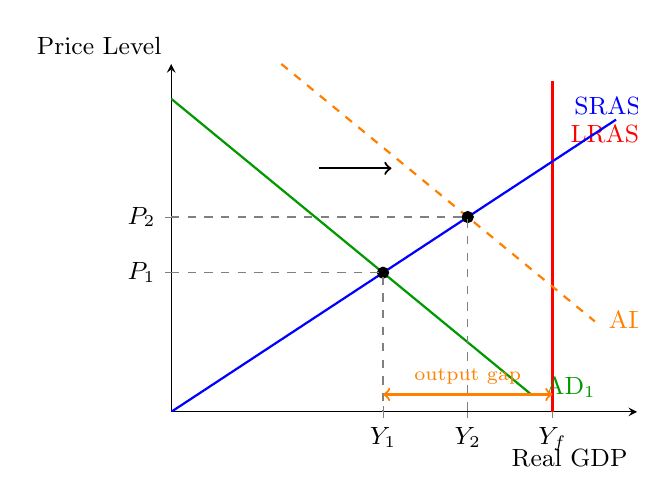
\begin{tikzpicture}
                    \begin{axis}[
                        axis lines = middle,
                        xlabel = {Real GDP},
                        ylabel = {Price Level},
                        xmin=0, xmax=11, ymin=0, ymax=10,
                        xtick={5, 7, 9},
                        xticklabels={$Y_1$, $Y_2$, $Y_f$},
                        ytick={4, 5.6},
                        yticklabels={$P_1$, $P_2$},
                        width=7.5cm, height=6cm,
                        xlabel style={at={(axis description cs:1,0)}, anchor=north east, yshift=-10pt, font=\small},
                        ylabel style={at={(axis description cs:0,1)}, anchor=south east, font=\small},
                        tick label style={font=\small},
                    ]
                    % LRAS at Yf=9
                    \addplot[red, thick] coordinates {(9,0) (9,9.5)};
                    \node[red, font=\small, anchor=west] at (axis cs: 9.2, 8.0) {LRAS};
                    % SRAS: P = 0.8Y
                    \addplot[blue, thick, domain=0:10.5] {0.8*x};
                    \node[blue, font=\small] at (axis cs: 10.3, 8.8) {SRAS};
                    % AD1: P = 9 - Y  (E1 at Y=5, P=4); label at right end of curve
                    \addplot[green!60!black, thick, domain=0:8.5] {9 - x};
                    \node[green!60!black, font=\small, anchor=west] at (axis cs: 8.6, 0.7) {AD$_1$};
                    % AD2: P = 12.6 - Y  (E2 at Y=7, P=5.6); label at right end of curve
                    \addplot[orange, thick, dashed, domain=2.6:10] {12.6 - x};
                    \node[orange, font=\small, anchor=west] at (axis cs: 10.1, 2.6) {AD$_2$};
                    % AD shift arrow (midway between the two curves)
                    \draw[->, thick, black] (axis cs: 3.5, 7.0) -- (axis cs: 5.2, 7.0);
                    % Equilibrium points (on SRAS at calculated intersections)
                    \coordinate (E1) at (axis cs: 5, 4);
                    \coordinate (E2) at (axis cs: 7, 5.6);
                    \filldraw (E1) circle (2pt);
                    \filldraw (E2) circle (2pt);
                    % Dashed reference lines from E1
                    \draw[dashed, gray] (axis cs: 0, 4)  -- (E1) -- (axis cs: 5, 0);
                    % Dashed reference lines from E2
                    \draw[dashed, gray] (axis cs: 0, 5.6) -- (E2) -- (axis cs: 7, 0);
                    % Output gap bracket at base
                    \draw[<->, thick, orange]
                        (axis cs: 5, 0.5) -- node[above, font=\scriptsize]{output gap} (axis cs: 9, 0.5);
                    \end{axis}
                \end{tikzpicture}
            \end{center}
        \end{column}
        \begin{column}{0.42\textwidth}
            \textbf{When AD rises (AD$_1 \to$ AD$_2$):}
            \begin{itemize}\setlength\itemsep{0.35em}
                \item Real GDP rises: $Y_1 \to Y_2$
                \item Economy moves toward $Y_f$
                \item Cyclical unemployment falls
                \item Price level rises: $P_1 \to P_2$
            \end{itemize}
            \vspace{0.5em}
            \textbf{When AD falls:}
            \begin{itemize}
                \item Output falls below $Y_f$
                \item Negative output gap opens
                \item Cyclical unemployment rises
            \end{itemize}
        \end{column}
    \end{columns}
\end{frame}

% ---- Global Factors ----------------------------------------
\begin{frame}{How Global Changes Affect UK Unemployment}
    The UK is an open economy --- events abroad directly affect UK employment.

    \vspace{0.3em}
    \begin{table}
        \centering
        \small
        \renewcommand{\arraystretch}{1.15}
        \begin{tabular}{@{}p{5.0cm}p{6.2cm}@{}}
            \toprule
            \textbf{Global event} & \textbf{Effect on UK unemployment} \\ \midrule
            Recession in trading partners & UK export demand falls $\Rightarrow$ manufacturing jobs lost \\
            Rise in commodity prices & Firms' costs rise $\Rightarrow$ output and employment fall \\
            Global financial crisis (2008) & Credit collapse $\Rightarrow$ AD falls $\Rightarrow$ cyclical unemployment surges \\
            Growth in low-cost manufacturing & UK industries undercut $\Rightarrow$ structural unemployment rises \\
            Strong global growth & Higher export demand $\Rightarrow$ UK employment rises \\ \bottomrule
        \end{tabular}
    \end{table}
\end{frame}

% ---- Global: Exchange Rate Link ----------------------------
\begin{frame}{The Exchange Rate Channel}
    \textbf{Exchange rate changes transmit global conditions into UK employment:}

    \vspace{0.5em}
    \begin{columns}
        \begin{column}{0.47\textwidth}
            \textbf{Sterling depreciates ($\pounds \downarrow$):}
            \begin{itemize}
                \item UK exports become cheaper abroad
                \item Demand for UK goods rises
                \item Export-sector employment rises
                \item Imports become more expensive $\Rightarrow$ import-competing firms benefit
            \end{itemize}
        \end{column}
        \begin{column}{0.47\textwidth}
            \textbf{Sterling appreciates ($\pounds \uparrow$):}
            \begin{itemize}
                \item UK exports become more expensive
                \item Overseas demand for UK goods falls
                \item Export-sector employment falls
                \item Cheap imports undercut UK producers
            \end{itemize}
        \end{column}
    \end{columns}

    \vspace{0.5em}
    \begin{example}
        After the Brexit referendum in 2016, sterling fell sharply. UK exporters became more competitive and some firms reported increased orders, supporting employment in manufacturing.
    \end{example}
\end{frame}

% ---- Symptoms, Diagnosis, Prescription ---------------------
\begin{frame}{Symptoms, Diagnosis, Prescription}
    \textbf{A useful framework for tackling unemployment policy questions:}

    \vspace{0.6em}
    \begin{columns}
        \begin{column}{0.30\textwidth}
            \textbf{Symptoms}\\
            \small What does the data show?\\
            Rising claimant count? High LFS rate? Regional concentration? Youth unemployment?
        \end{column}
        \begin{column}{0.30\textwidth}
            \textbf{Diagnosis}\\
            \small What type of unemployment is this?\\
            Frictional? Structural (skill/regional mismatch)? Cyclical (AD falling)?
        \end{column}
        \begin{column}{0.30\textwidth}
            \textbf{Prescription}\\
            \small What policy is appropriate?\\
            Supply-side (training, mobility)? Demand-side (fiscal/monetary stimulus)?
        \end{column}
    \end{columns}

    \vspace{0.8em}
    \begin{keypoint}
        A demand-side stimulus will not cure structural unemployment. A retraining programme will not cure cyclical unemployment. Match the policy to the diagnosis.
    \end{keypoint}
\end{frame}

% ---- Case Study: Port Talbot --------------------------------
\begin{frame}{Case Study: Tata Steel, Port Talbot (2024)}
    \textbf{Symptoms:}
    \begin{itemize}
        \item 2,800 job losses as two blast furnaces close; few alternative large employers in the area
    \end{itemize}

    \vspace{0.2em}
    \textbf{Diagnosis:}
    \begin{itemize}
        \item \textbf{Structural} --- global overcapacity, cheap overseas competition, high UK energy costs
        \item Skills are steel-specific; occupational and geographical mobility are both low
    \end{itemize}

    \vspace{0.2em}
    \textbf{Prescription:}
    \begin{itemize}
        \item Government retraining programmes for displaced workers
        \item Regional investment to attract alternative employers
        \item Subsidy for transition to electric arc furnace technology
    \end{itemize}

    \vspace{0.2em}
    \alert{Note:} A demand-side stimulus would not solve this --- the problem is structural, not cyclical.
\end{frame}

% ---- Activity ----------------------------------------------
\begin{frame}{Activity: Symptoms, Diagnosis, Prescription}
    \textbf{For each scenario, identify the type of unemployment, explain why, and suggest an appropriate policy:}

    \begin{enumerate}\setlength\itemsep{0.4em}
        \item UK interest rates rise sharply; consumer spending falls; retail firms announce redundancies.
        \item A wave of AI tools replaces data-entry and administrative roles across industries.
        \item A ski resort in Scotland lays off 40 staff in April as the season ends.
        \item A recent graduate spends 10 weeks looking for a marketing role before accepting an offer.
        \item A recession in Germany, the UK's largest export market, reduces orders for UK car parts.
    \end{enumerate}
\end{frame}

% ---- Summary -----------------------------------------------
\begin{frame}{Summary}
    \begin{itemize}\setlength\itemsep{0.35em}
        \item Two UK measures: \textbf{claimant count} (benefit claimants, distorted by rules) and \textbf{LFS/ILO} (preferred headline measure, internationally comparable)
        \item Four types: \textbf{frictional} (search frictions), \textbf{structural} (skill/geographic mismatch), \textbf{cyclical} (AD deficiency), \textbf{seasonal} (predictable variation)
        \item \textbf{Demand-side} causes: falls in C, I, G, or X reduce output and employment
        \item \textbf{Supply-side} causes: immobility, skill mismatches, poor information
        \item \textbf{Global} factors: recessions abroad, commodity prices, exchange rate changes all affect UK employment through the trade and financial channels
        \item \textbf{Policy must match the cause}: supply-side tools for structural/frictional; demand-side tools for cyclical
    \end{itemize}
\end{frame}

% ---- Key Terms ---------------------------------------------
\begin{frame}{Key Terms}
    \begin{description}
        \item[Claimant count] Number of people claiming unemployment-related benefits
        \item[LFS (ILO)] Without work, actively sought in last 4 weeks, available to start in 2 weeks
        \item[Frictional] Short-term search unemployment between jobs
        \item[Structural] Long-run mismatch of skills/location due to industry decline
        \item[Cyclical] Unemployment caused by deficient aggregate demand
        \item[Seasonal] Predictable variation in labour demand by time of year
        \item[Demand-side factors] Changes in AD components (C, I, G, X$-$M) affecting employment
        \item[Supply-side factors] Immobility, skill gaps, information failures in the labour market
        \item[Negative output gap] Actual GDP below productive potential; associated with cyclical unemployment
    \end{description}
\end{frame}

\end{document}
